\chapter{Pruebas}

\section{Teléfonos utilizados}

Para comprobar y asegurar el correcto funcionamiento de la aplicación en el mayor número de casos posibles, hemos utilizado diferentes dispositivos móviles con características dispares de software, tamaño de pantalla, densidad de píxeles o tamaño de fuente, entre otras.

En concreto, los teléfonos utilizados han sido:

\begin{table}[H]
\centering
\begin{tabular}{|l|l|l|l|l}
\cline{1-4}
\textbf{Marca} & \textbf{Modelo} & \textbf{Versión de software} & \textbf{Pantalla} & \\ \cline{1-4}
    Google & Pixel XL & API 28 (Android 9 Pie) & 5,5" &  \\ \cline{1-4}
    Google & Pixel XL & API 29 (Android 10) & 5,5" &  \\ \cline{1-4}
    Huawei & ALE-L21 & API 23 (Android 6.0 Marshmallow) & 5" &  \\ \cline{1-4}
    Xiaomi & Mi A2 Lite & API 28 (Android 9 Pie) & 5,84", notch &  \\ \cline{1-4}
    Nexus  & 5 & API 21 (Android 5 Lollipop) & 4,95" &  \\ \cline{1-4}
    ZTE  & BLADE A512 & API 23 (Android 5 Lollipop) & 5,2" &  \\ \cline{1-4}
\end{tabular}
\end{table}

No todos los teléfonos tienen además la misma forma de pantalla. Es el caso del Xiaomi Mi A2 Lite, cuya pantalla es bastante más alargada y menos ancha que la del resto de dispositivos. 

Por otra parte, tanto el Xiaomi recién mencionado como el Huawei ALE-L21 son utilizados con el máximo tamaño de texto permitido. En el caso del ZTE BLADE, la resolución de pantalla (densidad de píxeles) no es muy alta, lo que provoca que todos los elementos aparezcan con una mayor dimensión. Tener estos datos en cuenta es importante para comprobar que el diseño de la interfaz no se desorganiza, provocando solapamientos en las cadenas de texto o desbordamientos fuera de pantalla que impedirían la correcta visualización de información. 

Salvo los problemas que comentaremos en el siguiente apartado, todo funciona correctamente en cada uno los móviles de la tabla superior, asegurando el correcto funcionamiento del proyecto en un bastante amplio rango de dispositivos.

\section{Problemas en otros dispositivos}

\subsection{Visualización incorrecta de algunas imágenes}

En algunas versiones de Android con una API inferior a 23, se presentaba un extraño error que provocaba la incorrecta visualización de imágenes vectoriales, imágenes que sí se veían correctamente en el resto de dispositivos.

Parece ser un fallo más o menos común. Tras distintos intentos, la única forma de solucionarlo ha sido sustituir las imágenes vectoriales afectadas por su versión en formato PNG, el cual muestra las imágenes tal y como fueron diseñadas. La contrapartida de esta decisión es que el tamaño de los recursos PNG es muy superior al de los vectoriales, a lo que hay que añadir la necesidad en Android de incorporar múltiples versiones de la misma imagen con distintas resoluciones para evitar que pierdan calidad en pantallas más grandes.

\begin{figure}[H]
	\centering
	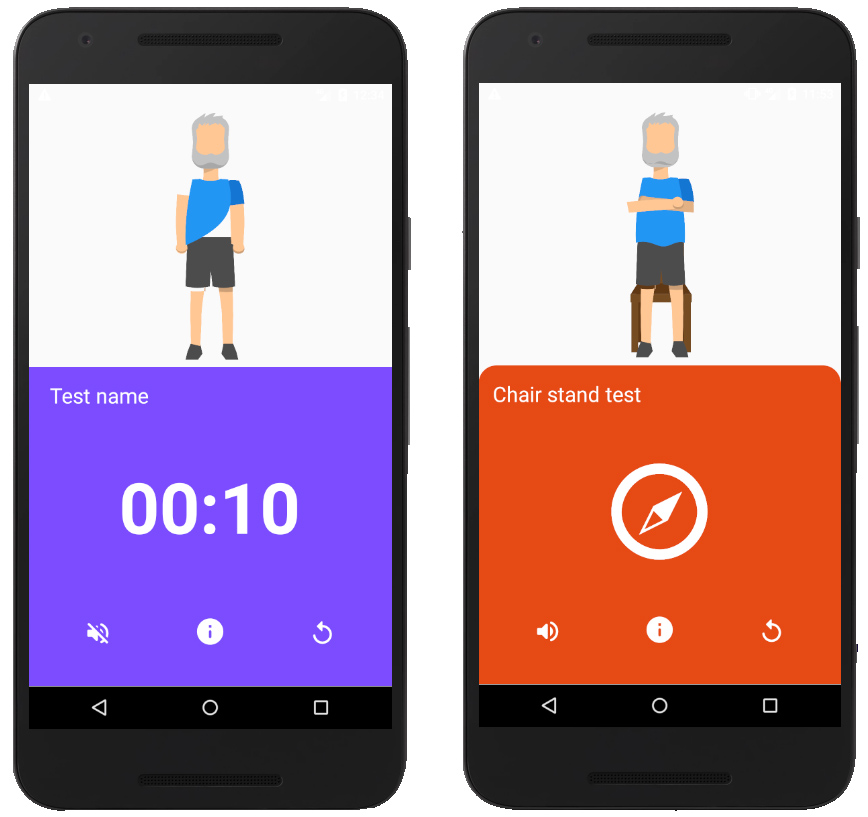
\includegraphics[scale=0.30]{imagenes/errores.jpg}
	\caption{Errores de visualización vectorial.\label{fig:errores}}
\end{figure}

\subsection{Periodos de muestreo diferentes}

El periodo o frecuencia de muestreo es el tiempo que transcurre entre que el servicio de acelerómetro ofrece un dato y el siguiente. 

Durante el desarrollo de la aplicación se había establecido un periodo de muestreo de 1Hz, es decir, se pretendía obtener los datos del acelerómetro cada 1 segundo. Sin embargo, esta frecuencia no se cumplía de igual forma en todos los dispositivos de la tabla anterior, lo que provocó que mientras la evaluación de las pruebas se llevaba a cabo de forma correcta en el teléfono de desarrollo (Google Pixel XL), el funcionamiento fuese totalmente impredecible en otros.

Veamos algunos comportamientos concretos. En el teléfono Xiaomi Mi A2 Lite la tasa de muestreo estaba siendo muy superior a la establecida, llegando a devolver la aceleración que se conseguía cada pocas milésimas de segundo. Como es de imaginar, la aceleración acumulada que se produce entre dos espacios de tiempo muy cercanos será menor que la que se produce entre dos espacios de tiempo separados por un segundo. Esta aceleración, al ser tan pequeña, es muy fácil de igualar incluso sin moverse (como resultado del ruido en los datos), lo que convertía la prueba de levantarse y sentarse en la silla en un conjunto de errores sin la más mínima fiabilidad puesto que constantemente determinaba que el usuario se había levantado y sentado.

Por otra parte, el teléfono Huawei ALE-L21 tenía un periodo de muestreo muy lento, lo que impedía por completo el funcionamiento de las tres pruebas. 

Finalmente, el problema se resolvió estableciendo una tasa de refresco por defecto (\textit{sensor\_delay\_game}) en todos los tests, y controlando mediante un condicional \textit{if} que no se accede a la información del acelerómetro hasta que no ha transcurrido un tiempo mínimo de 100 milisegundos. 

\begin{lstlisting}
sensorManager.registerListener(this, sensorAcc, SensorManager.SENSOR_DELAY_GAME);
\\ ...
if ((System.currentTimeMillis() - lastSaved) > ACCE_FILTER_DATA_MIN_TIME) {
    \\ ... 
}
\end{lstlisting}

\subsection{Falta de soporte de características visuales}

En las versiones de software más bajas soportadas por la aplicación, hay determinados elementos estéticos que no pueden visualizarse por falta de soporte. Un ejemplo es el color personalizado de la barra de estado para dispositivos con API 21, que se utiliza en toda la aplicación para mostrarla del mismo color blanco que el fondo, o de una tonalidad más oscura del color correspondiente en la actividad de instrucciones.

\section{Pruebas en usuarios}

Se han llevado a cabo pruebas sobre usuarios reales para la persecución de múltiples objetivos. 

Por una parte, durante la evolución individual de cada uno de los algoritmos de medición, era necesario poner a prueba continuamente los avances en el proyecto, tarea que ha recaído principalmente sobre el desarrollador. A medida que estos algoritmos abandonaban el estado de desarrollo para acercarse al de producción, han sido otros usuarios con diferentes edades (comprendidas entre los 20 y los 60 años) los que han participado en las pruebas.

Se les ha pedido usar la aplicación de forma autónoma, una actividad muy útil de cara a estudiar, por ejemplo, dificultades entendiendo el funcionamiento de la interfaz.

\begin{figure}[H]
	\centering
	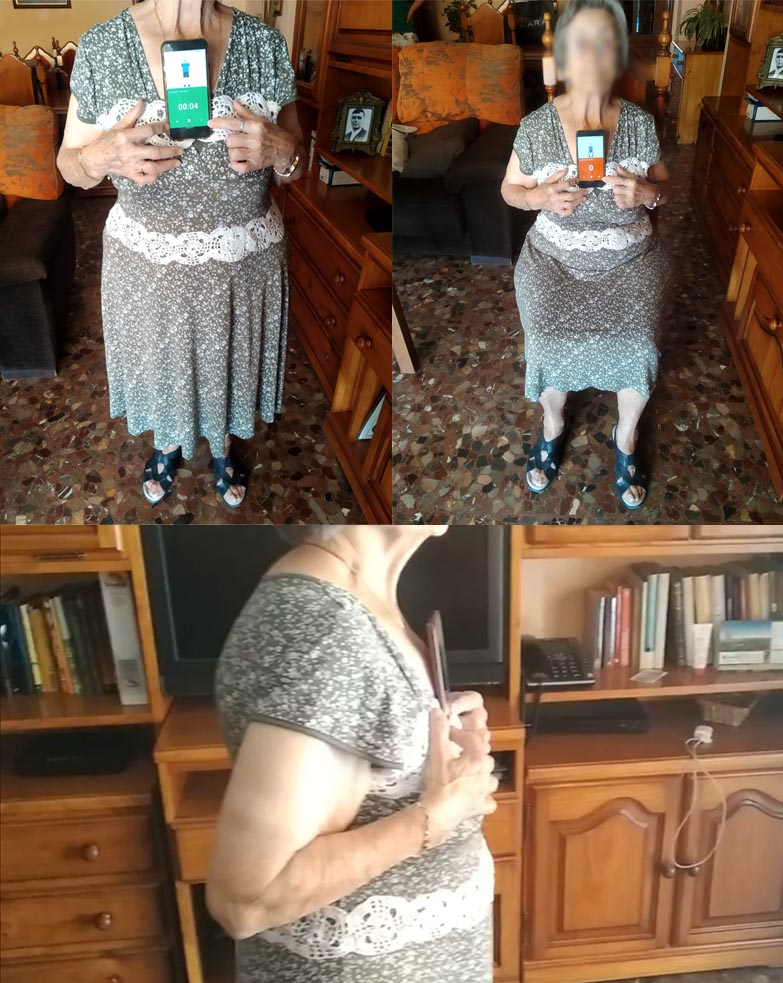
\includegraphics[scale=1.5]{imagenes/pruebas.jpg}
	\caption{Pruebas con ancianos.\label{fig:pruebas_mayores}}
\end{figure}

A medida que se localizaban errores durante la utilización con usuarios reales, se tomaban medidas para corregirlos o adaptarlos. De este modo se han pulido diversos aspectos de la aplicación hasta alcanzar un estado apto para pruebas con personas más mayores (más de 85 años) como se puede ver en la figura superior \ref{fig:pruebas_mayores}.

En general, los resultados obtenidos mediante las pruebas llevadas a cabo en las últimas fases del desarrollo de la \textit{app} han sido satisfactorios. Los usuarios comprendían de forma aceptable cómo navegar por la interfaz y las instrucciones para la realización de los tests. Además, las mediciones eran correctas en la mayoría de casos a excepción del test de \textit{levantarse de la silla con el móvil en el pecho}, el cual deberá sufrir aún más mejoras.

Estas pruebas no se han empleado para ningún propósito más allá del de mejorar y enriquecer el proyecto. Por tanto, no nos hemos ocupado de crear estadísticas de errores surgidos tanto en la ejecución como en el manejo de la aplicación.

Se espera, no obstante, una colaboración con el Departamento de Enfermería y Fisioterapia de la Universidad de Cádiz y con el Institute of Artificial Intelligence de De Montfort University en Leicester (Reino Unido) para validar los resultados con más usuarios reales durante los próximos meses.
